\section{Load Balancer Resource Usage}
\subsection{Resource Evaluation Setup}
% 2 pages -> got 4
The goal of these experiments is to understand the resource consumption one can expect from a load balancer in the context of serverless edge computing.
Using the traces of these experiments we implement the load balancers within the serverless simulator as close to reality as possible, thus making sure the simulation results are more representative.

As described we use a Kubernetes cluster with a number of different nodes to make real-life measurements of load balancer's performance characteristics, requests are sent via galileo\cite{galileo-github}\cite{operating-energy-aware-galileo}, and the system metrics are measured via telemd\cite{telemd-github}.
Since the load balancer is containerized, just like it would be in a serverless framework, telemd relies on the metrics provided by Kubernetes to measure resource consumption.
Specifically, telemd reports the values provided by the following files at a set interval\cite{telemd-github}.
\begin{lstlisting}[language=Bash]
/sys/fs/cgroup/cpuacct/kubepods/besteffort/pod<pod ID>/<container ID>/cpuacct.usage
/sys/fs/cgroup/memory/kubepods/besteffort/pod<pod ID>/<container ID>/memory.stat
\end{lstlisting}
Network characteristics are not taken into account with these measurements, as they are highly application specific and experimental evaluation is thus neither fruitful nor necessary.

Since scaling and scheduling are important aspects of our approach, we also consider the image size of the load balancer to be relevant.
Because Docker Hub is one of the largest hosting platforms for application container images, we use the information it provides\cite{traefik-dockerhub} to determine the image size for different platforms.

To cover a wide range of possible deployment scenarios the nodes we use for this experiment cover hardware from powerful desktop processors as they are used in large scale data centers to small scale reduced instruction set processors as one finds in mobile devices.

\begin{table}[]
\begin{tabular}{lllll}
\hline
\textbf{Node} & \textbf{\begin{tabular}[c]{@{}l@{}}Processor\\ Architecture\end{tabular}} & \textbf{\begin{tabular}[c]{@{}l@{}}logical CPU\\ core count\end{tabular}} & \textbf{\begin{tabular}[c]{@{}l@{}}RAM\\ (GiB)\end{tabular}} & \textbf{Model Name}           \\ \hline
AMD           & x86/amd64                                                                 & 8                                                                         & 32                                                           & AMD Ryzen Embedded V1605B     \\
Intel         & x86/amd64                                                                 & 8                                                                         & 16                                                           & Intel Xeon E3-1230 v6         \\
Jetson        & aarch64                                                                   & 4                                                                         & 4                                                            & NVIDIA Jetson Nano            \\
RockPi        & aarch64                                                                   & 6                                                                         & 4                                                            & RockPi 4B                     \\
RPi           & ARMv7                                                                     & 4                                                                         & 1                                                            & Raspberry Pi 4Model B Rev 1.1
\end{tabular}
\caption{Nodes present in the real Kubernetes cluster used for resource consumption evaluation}
\label{tab:k8s_nodes}
\end{table}



Table \ref{tab:k8s_nodes} shows the different nodes that are present in the cluster and which get evaluated. Aside from covering typical compute resources we also include a number of ARM devices, one with special purpose compute acceleration, to show how mobile edge computing devices or devices built for purposes such as image processing would perform.

To evaluate load balancer's resource consumption we need to select a real load balancer implementation that serves as a stand-in for generic load balancers.
For this purpose we selected traefik proxy\cite{traefik}, a level 7 load balancer and application proxy.
We considered it a fitting example of a real world load balancer since it is available on all the different platforms we want to test, supports the kind of complex load balancing required of our proposed approach.
It is also open source, which allowed us to extend it with least response time load balancing capabilities like we proposed, which further moves these experiments closer to real-world conditions.
This modified version\cite{traefik-jjnp} is also open source and is already functional, although it does not feature the integrations that would allow its use in a serverless framework.

Since in the experimental setup requires actual requests being sent we also need an upstream the load balancer can then forward the requests it receives to.
For this experiment the upstream is a separate application that does nothing but respond to the requests with a given payload.
Its only distinguishing feature is that we can choose from a random distribution that determines how long the application waits before responding, thus simulating the \gls{fet} usually experienced within a serverless system.
For the general evaluation of different devices we simulated a response time/\gls{fet} of 20 milliseconds.
We built this application specifically for this purpose, and also made it publicly available\cite{palecekResponder2021} so that it can be used by others.
We oriented our payload on a hypothetical edge intelligence application, where a client sends an image for it to then be classified.
Our payload is thus a compressed JPEG image with a file size of 250KiB, while the response is a simple JSON with negligible size.

Lastly for the request load we decided to test a range of different loads.
To do this in a simple and presentable way we send requests along a pattern, which steadily increases the amount of requests sent from 0 to 250 requests per second over a period of 300 seconds, then continuously sending 250 requests per second for 60 more seconds before stopping completely.

Apart from the evaluation of different types of devices we performed another test with the same request pattern, but one time with the previously used response time of 20ms and once again with a response time of 250ms to see whether the response time of the upstreams makes a difference to the load balancer resource consumption.
\subsection{Observed Resource Consumption}
Our results show that the resource consumption of load balancers of this class is, generally speaking, quite moderate.
At a rate of 250 requests per seconds, a substantial load, CPU utilization ranges from 4,3\% to 34\%, while memory consumption is between 12 and 59MiB.
The results at 250 requests per second can be seen in Table \ref{tab:resource_eval_results}.

The relationship between the resource consumption and request load can be seen in Figure \ref{fig:lb_resources_by_type}.
From these graphs we can see that CPU utilization rises almost linearly with the number of concurrent requests, while the RAM consumption does not show a comparable pattern.
In fact, the memory consumption shows significant variance between the different nodes with some nodes showing more than quadruple the system memory usage of others.
There is also no obvious explanatory pattern to be observed, as these wide ranges of memory consumption also exist within nodes of the same processor architecture.

The response time of the upstream services also appears to influence resource utilization as can be seen in Figure \ref{fig:lb_resources_by_rt}.
While the CPU utilization seems to be consistent throughout the experiments with 20ms and 250ms response time, the memory consumption is higher for the case of 250ms.

Lastly, the size of the different Docker images, which can be seen in Table \ref{tab:resource_eval_results}, does differ across processor architectures, but not to a significant degree.
The difference between the largest and the smallest images is 2,28Mib, or 8\% to 8,5\%, depending on which image is considered the default basis for the calculation.


\begin{table}[]
\begin{tabular}{lrrr}
\hline
\textbf{Node} & \textbf{CPU utilization} & \textbf{RAM Usage} & \textbf{Docker Image Size} \\ \hline
AMD           & 4,3\%                    & 57 MiB             & 28.46 MB                   \\
Intel         & 6,5\%                    & 16 MiB             & 28.46 MB                   \\
Jetson Nano   & 12,5\%                   & 16 MiB             & 26.18 MB                   \\
RockPi        & 13\%                     & 59 MiB             & 26.18 MB                   \\
RPi           & 34\%                     & 12 MiB             & 26.75 MB                  
\end{tabular}
\caption{Results of the load balancer resource evaluation at 250 requests per second}
\label{tab:resource_eval_results}
\end{table}
\begin{figure}
    \centering
    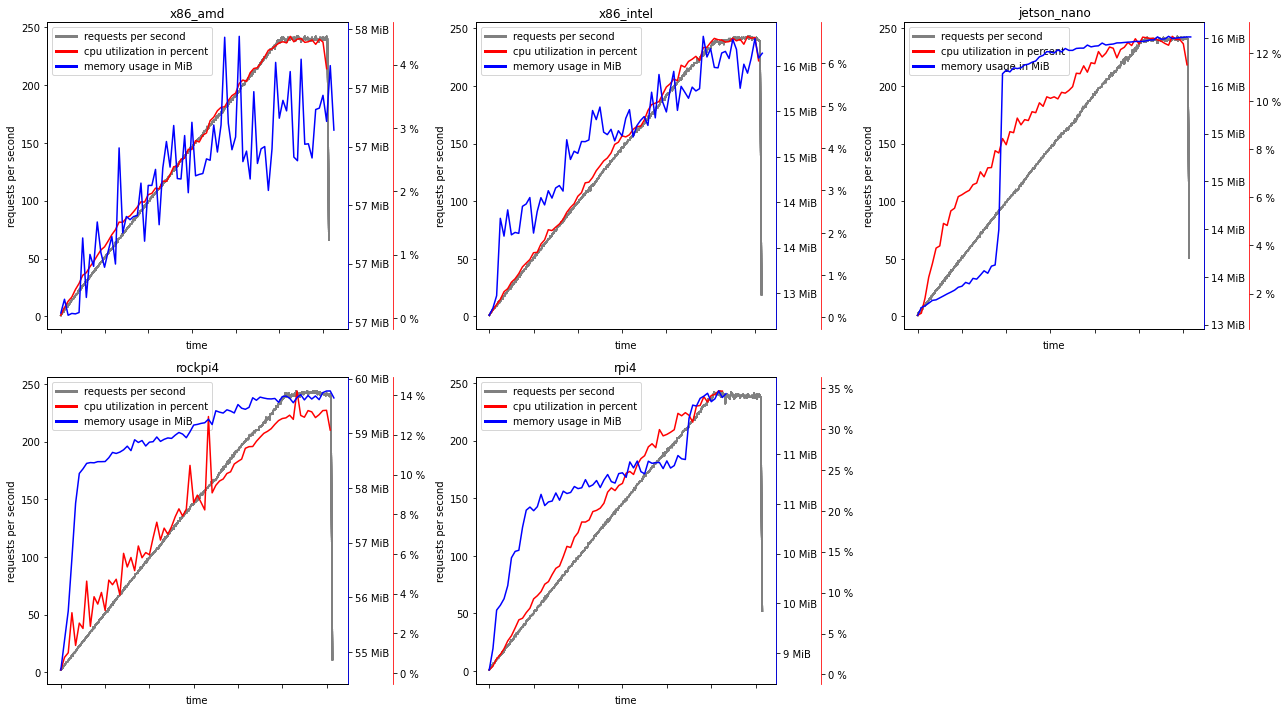
\includegraphics[width=14cm]{graphics/graphs/lb_resources_by_device.png}
    \caption{Resource consumption of the traefik\cite{traefik} load balancer on different devices with a response time of 20ms and request payload size of 250KiB}
    \label{fig:lb_resources_by_type}
\end{figure}

\begin{figure}
    \centering
    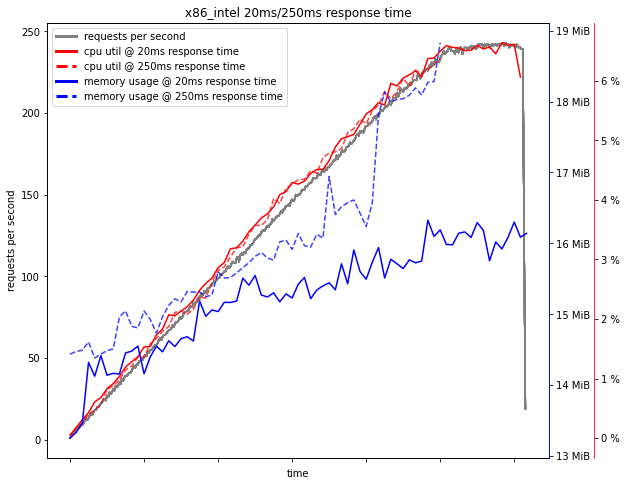
\includegraphics[width=11cm]{graphics/graphs/lb_resources_by_response_time.png}
    \caption{Resource consumption of the traefik\cite{traefik} load balancer with different response times on and a 250KiB request payload}
    \label{fig:lb_resources_by_rt}
\end{figure}
